\documentclass[12pt,letterpaper,noanswers]{exam}
\usepackage[usenames,dvipsnames,svgnames,table]{xcolor}
\usepackage[margin=0.9in]{geometry}
\usepackage{tikz}
\renewcommand{\familydefault}{\sfdefault}
\usepackage{multicol}
\pagestyle{head}
\definecolor{c03}{HTML}{FFDDDD}
\header{AM 111 Class 24}{}{Skill Check}
\runningheadrule
\headrule
\usepackage{graphicx} % more modern
\usepackage{amsmath} 
\usepackage{amssymb} 
\usepackage{hyperref}
\usepackage{tcolorbox}

\begin{document}
 \pdfpageheight 11in 
  \pdfpagewidth 8.5in

\noindent Name: \rule{2.5in}{0.5pt}

\noindent Put away any notes or other materials, and work on this activity alone.

\noindent You'll receive feedback on your work and will complete a similar question on a future skill check.


\begin{questions}

\item (Retake for Class 22)

Match the signal to its DFT amplitude.  Provide reasoning.

Signal:

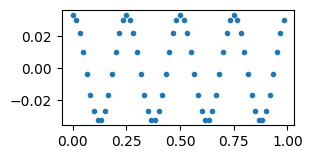
\includegraphics[width=0.3\linewidth]{img/C21skill-2.png}

Frequency options:

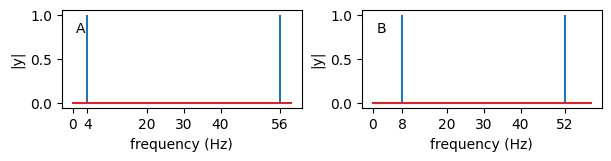
\includegraphics[width=0.7\linewidth]{img/C21skill2-2.png}
\vspace{3cm}
\item (Retake for Class 23)

For the neural network below, how many inputs does it have?  How many units in the first hidden layer?  What is the depth of the network?

\newcommand{\inputnum}{3} 
% Hidden layer neurons'number
\newcommand{\hiddennum}{6} 
% Hidden layer neurons'number
\newcommand{\hiddennumk}{4}
% Output layer neurons'number
\newcommand{\outputnum}{2} 
\begin{tikzpicture}
% Input Layer
\foreach \i in {1,...,\inputnum}
{
    \node[circle, 
        minimum size = 6mm,
        fill=orange!30] (Input-\i) at (0,-\i) {};
}
% Hidden Layer
\foreach \i in {1,...,\hiddennum}
{
    \node[circle, 
        minimum size = 6mm,
        fill=teal!50,
        yshift=(\hiddennum-\inputnum)*5 mm
    ] (Hidden-\i) at (2.5,-\i) {};
}
\foreach \i in {1,...,\hiddennumk}
{
    \node[circle, 
        minimum size = 6mm,
        fill=teal!50,
        yshift=(\hiddennumk-\inputnum)*5 mm
    ] (Hiddenk-\i) at (5,-\i) {};
}
% \foreach \i in {1,...,\hiddennumm}
% {
%     \node[circle, 
%         minimum size = 6mm,
%         fill=teal!50,
%         yshift=(\hiddennumm-\inputnum)*5 mm
%     ] (Hiddenm-\i) at (7.5,-\i) {};
% }
% Output Layer
\foreach \i in {1,...,\outputnum}
{
    \node[circle, 
        minimum size = 6mm,
        fill=purple!50,
        yshift=(\outputnum-\inputnum)*5 mm
    ] (Output-\i) at (7.5,-\i) {};
}
% Connect neurons In-Hidden
\foreach \i in {1,...,\inputnum}
{
    \foreach \j in {1,...,\hiddennum}
    {
        \draw[->, shorten >=1pt] (Input-\i) -- (Hidden-\j);   
    }
}
% Connect neurons Hidden-Out
\foreach \i in {1,...,\hiddennum}
{
    \foreach \j in {1,...,\hiddennumk}
    {
        \draw[->, shorten >=1pt] (Hidden-\i) -- (Hiddenk-\j);
    }
}
% \foreach \i in {1,...,\hiddennumk}
% {
%     \foreach \j in {1,...,\hiddennumm}
%     {
%         \draw[->, shorten >=1pt] (Hiddenk-\i) -- (Hiddenm-\j);
%     }
% }
\foreach \i in {1,...,\hiddennumk}
{
    \foreach \j in {1,...,\outputnum}
    {
        \draw[->, shorten >=1pt] (Hiddenk-\i) -- (Output-\j);
    }
}
% Inputs
\foreach \i in {1,...,\inputnum}
{     
    \draw (Input-\i) node {$x_{\i}$};
    % \draw[<-, shorten <=1pt] (Input-\i) -- ++(-0.5,0)
    %     node[left]{$x_{\i}$};
}
% Outputs
\foreach \i in {1,...,\outputnum}
{            
\draw (Output-\i) node {$y_{\i}$};
    % \draw[->, shorten <=1pt] (Output-\i) -- ++(0.5,0)
    %     node[right]{$y_{\i}$};
}
\end{tikzpicture}


\end{questions}

\end{document}
